\documentclass{article}

\usepackage[utf8]{inputenc}
\usepackage[french]{babel}
\usepackage{mathtools}
\usepackage{amssymb}
\usepackage{tikz}
\usetikzlibrary{matrix}
\usepackage{url}
\usepackage{enumitem}
\usepackage{multicol}
\usepackage{hyperref}

\hypersetup{
    colorlinks,
    citecolor=green,
    filecolor=blue,
    linkcolor=blue,
    urlcolor=blue
}

\usepackage{graphicx}
\newtheorem{theorem}{Théorème}
\newtheorem{lemma}{Lemme}
\newtheorem{corolaire}{Corollaire}
\newtheorem{proposition}{Proposition}
\newtheorem{definition}{Définition}
\newenvironment{proof}{{\sc Preuve:}}{~\hfill C.Q.F.D.}
\newenvironment{AMS}{}{}
\newenvironment{keywords}{}{}

\usepackage{epigraph}

% \epigraphsize{\small}% Default
\setlength\epigraphwidth{8cm}
\setlength\epigraphrule{0pt}

\usepackage{etoolbox}

\makeatletter
\patchcmd{\epigraph}{\@epitext{#1}}{\itshape\@epitext{#1}}{}{}
\makeatother

\title{Projet d'informatique semestre 3}
\author{Félix Desmaretz \& Maxime Flin}
\date{}

\begin{document}
\maketitle

Ce document est le compte rendu du projet de \textbf{programmation orienté objet et interface graphique} réalisé au troisième semestre de la licence d'informatique au cours de l'année 2017. Nous avons donc modélisé un jeu de l'oie et un jeu de numéri puis avons créé une interface graphique permettant de jouer en dehors de la console.
\tableofcontents
\newpage

\section{La modélisation}
Nous avons opté pour un modélisation basé sur un principe d'événements afin de rendre le jeu le plus modulable possible et d'exploiter une maximum les lambdas expressions apparuent dans Java8. 

L'organisation autour d'événement rend le jeu plus modulable dans le sens où il suffit d'écrire de petit script pour modéliser un comportement. De plus, ces scripts peuvent parfaitement se superposer et il est ainsi très simple, par exemple, de faire un case prison qui pose une question à chaque tour pouvant nous faire perdre des points.

Nous trouvons que l'utilisation de lambdas expression est un plus dans la lisibilité du code et dans l'architecture du projet qui, par conséquent reste assez légère puisque pas encombré par plein des classes héritées.

\subsection{Les événements}

Ainsi les événements que nous avons choisit d'ajouter sont les suivants:
\paragraph{Pour le joueurs}
\begin{enumerate}
\item Quand on commence son tour. C'est cet événement qui dit au joueur de lancer le dé et de déplacer ses pions.
\item Quand on fini tour. Quand un joueur termine son tour on test par exemple s'il a gagné
\item Quand on passe son tour. Quand on ne peux pas jouer on peut perdre des points, décrémenter un compteur de tour a attendre...
\end{enumerate}

\paragraph{Pour les cases}
\begin{enumerate}
\item Quand un pion entre sur la case. On peut, par exemple, tester si la case est déjà occupé auquel cas on envoie le pion sur la case suivante ou précédente. On peut poser une question au joueur dès qu'il arrive...
\item Quand un pion quitte la case. On peut changer l'état de la case d'occupé à libre.
\item Quand on reste sur la case. On peut décrémenter un nombre de tour à attendre.
\end{enumerate}

Toutes les actions du jeu sont basées sur l'implémentation de ces 6 événements qui sont déclenché par la classe Game.

\subsection{Les classes de base}

\paragraph{La classe $Game$} est une classe abstraite représentant une partie. Il est important de noter qu'on considère ici, qu'au cours d'une exécution du programme, il n'y a qu'une partie en cours à la fois. Ainsi la classe $Game$ demande d'implémenter les classes abstraites suivantes:

\begin{enumerate}
\item $setup$. Cette méthode à pour vocation de créer les cases du jeu et de placer tous les pions à leur position de départ.
\item $isEnd$. Cette méthode doit retourner vrai si le jeu est fini et faux sinon.
\end{enumerate}

Elle implémente l'interface $Iterable<Player>$ afin de pouvoir parcourir facilement les joueurs inscrits et a une classe interne $State$ qui permet d'interagir avec le jeu de partout. Cette dernière contient le cycle de joueur (càd l'ordre dans lequel les joueurs jouent) et permet d'influer dessus. $Game$ possède une instance statique de cette classe interne qui permet d'interagir avec elle partout.

Pour finir on trouve dans cette classe une instance de la classe $Board$, initialisé dans la méthode $start$, qui permet de modéliser la succession des tours.

\paragraph{Le $Board$} est une classe qui implémentais, au départ, l'interface $Iterable<Player>$ et qui permet modéliser la succession des tours. Elle a une classe interne Cycle qui représente le cycle de joueur, et qui implémentais au départ $Iterator<Player>$. La méthode $hasNext$ renvoie vrai tant qu'il y a des joueurs et la méthode $next$ renvoie le joueur suivant. 

J'ai pris la peine de préciser qu'a l'origine ces classes implémentais des itérateurs parce que nous avons du modifier cette interface décrit bien le comportement de notre cycle de joueur. L'inconvénient étant qu'un simple itérateur ne permet pas d'implémenter la suppression d'un joueur. Nous avons trouvé que $ListIterator$ nous permettais de le faire. Elle demandais cependant d'implémenter d'autres fonctionnalités qui ne nous étaient pas utiles et nous avons donc abandonné cet idée.

\paragraph{La classe $Player$} est une classe abstraite qui représente un joueur. Elle ne possède pas de méthode abstraire mais nous avons décidé de la faire quand même abstraite car elle ne possède pas de lien avec un Pion. Vous concevrez aisément que la place du joueur dans un jeu de plateau est alors assez réduite, et même inexistante pour notre cas. 

Elle possède néanmoins une classe interne qui implémente l'interface $ActionListener<Event>$ qui permet de recevoir et de déclencher des événements. Cette classe interne permet d'ajouter les actions à réaliser quand un joueur commence, fini ou passe son tour.

On trouve dans la classe $Player$ des classes internes qui représentent des comportements suffisamment "standard" pour l'avoir mis dans là. Elles modélisent le déplacement d'un pion par un lancé de dés.

La classe $Player$ possède deux sous classes: $GoosePlayer$ et $NumeriPlayer$ qui implémentent la relation entre le joueur et ses pions. Dans $GoosePlayer$ on trouve une fonction $getPawn$ qui renvoi un $Pawn$ et dans $NumeriPlayer$ une fonctions $pawns$ qui renvoi un tableau de $NumeriPawn$.

\paragraph{La classe $Pawn$} représente, comme son nom l'indique, un pion sur le plateau. C'est une classe assez vide. Elle possède une méthode $getLocation$ et $getPlayer$ qui renvoient respectivement l'instance de la case sur laquelle le pion se trouve et le joueur auquel il appartient. Et on trouve aussi la méthode $goToCell$ qui déplace le pion en prenant bien soin de déclencher les événements appropriés.

Dans le jeu de l'oie on utilise directement la classe $Pawn$ mais dans le numeri on utilise une sous classe $NumeriPawn$ qui possède un attribut entier constant qui correspond au numéro ce dernier porte.

\paragraph{La classe $Configuration$} a été ajouté assez tardivement. Elle permet de gérer le paramétrage du jeu. Elle possède des classes internes décrivant les différents paramètres du jeu de l'oie et du numeri.

L'instance de cette classe est statique et constante. C'est à dire que partout dans le projet on accède à la même instance de $Configuration$.

\begin{figure}
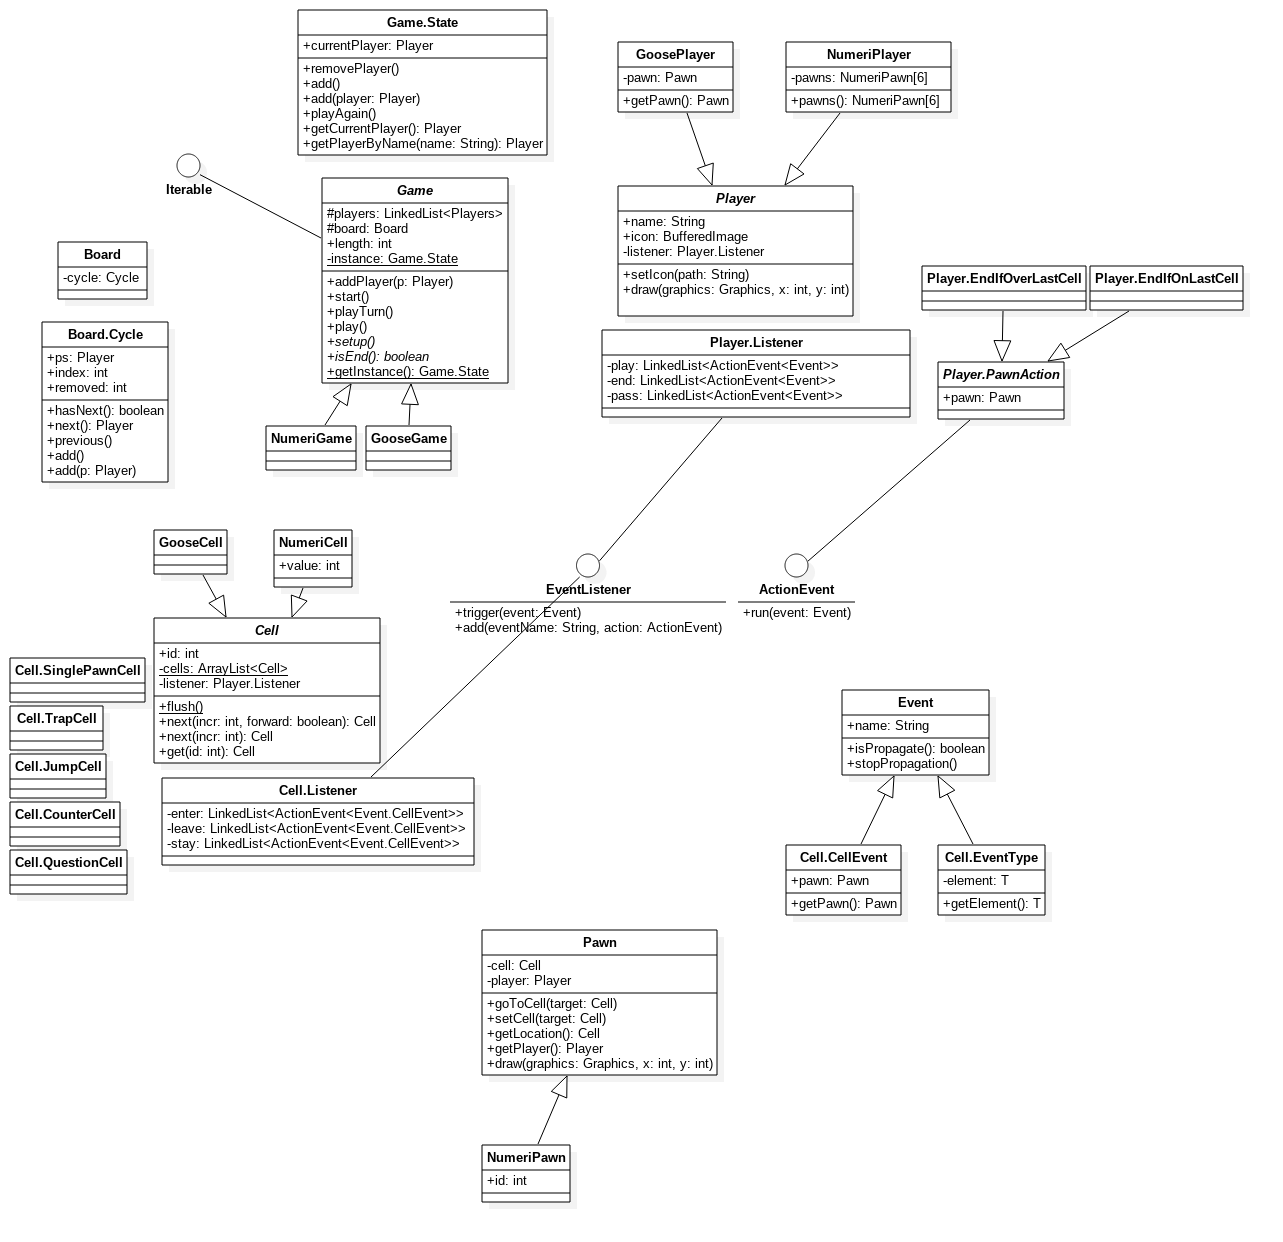
\includegraphics[width=\textwidth]{schema-uml.png}
\caption{
\textbf{Schéma du modèle.}
En carré les classes, en rond les interfaces, les champs précédés d'un $+$ sont publics, d'un $\#$ sont protected et d'un $-$ privés.}
\end{figure}

\section{L'interface graphique}
L'interface graphique fut de loin la partie la plus ennuyante et la plus longe de ce projet, ne devenant intéressante qu'au cours de quelques fulgurances pour lui donner un aspect personnel.

Dans le soucis d'écrire une code bien organisé, propre et facilement modifiable nous avons utilisé beaucoup de sous classes pour gérer les aspects graphiques puis avons définis les interactions dans la classe englobante. Malgré tout, nous considérons cet aspect de notre projet comme un échec car le code reste très confus et brouillon.

Le deuxième point qui devrait être retravailler est le design des éléments natif de java Swing, qui, bien qu'il ait été modifié, reste à notre gout assez décevant (pour les boutons par exemple).

Pour finir, je pense que nos animations (planètes qui tournent sur elles même, défilement du fond, météorites) sont très couteuses en performances. Il faudrait retravailler la mise en place des $Thread$ pour peut être n'en partager qu'un seul, qui devra surement, par conséquent, être statique, à l'image des météorites.

\section{Conclusion}
Pour conclure, nous pensons que ce projet aborde la modélisation du jeu sous un angle intéressant, assez peu présent certes dans java compte tenu de la grande expressivité de la programmation orienté objet, mais qu'on retrouve dans des langages plus récents comme $Javascript$ ou dans certains frameworks de développement de jeu vidéo, comme $Unity$.

Il y aurait, s'il fallait poursuivre, de nombreuses modifications à faire sur l'interface graphique avant d'avoir quelque chose de vraiment bon et dont nous pourrions être fier. Et nous pourrions ajouter sans trop de difficultés la possibilité de sauvegarder une partie, d'éditer complètement le plateau et de le partager avec ses amis. Le modèle étant fait en java on pourrais même envisager une version du jeu sous android (nous précisons bien envisager, je doute que l'envie vienne un jour).

\newpage
\nocite{*}

\bibliographystyle{plain}

\end{document}
